\documentclass[
	% -- opções da classe memoir --
	article,			% indica que é um artigo acadêmico
	12pt,				% tamanho da fonte
	oneside,			% para impressão apenas no recto. Oposto a twoside
	a4paper,			% tamanho do papel. 
	% -- opções da classe abntex2 --
	%chapter=TITLE,		% títulos de capítulos convertidos em letras maiúsculas
	%section=TITLE,		% títulos de seções convertidos em letras maiúsculas
	%subsection=TITLE,	% títulos de subseções convertidos em letras maiúsculas
	%subsubsection=TITLE % títulos de subsubseções convertidos em letras maiúsculas
	% -- opções do pacote babel --
	english,			% idioma adicional para hifenização
	brazil,				% o último idioma é o principal do documento
	sumario=tradicional
	]{abntex2}

\usepackage{lmodern}			% Usa a fonte Latin Modern
\usepackage[T1]{fontenc}		% Selecao de codigos de fonte.
\usepackage[utf8]{inputenc}		% Codificacao do documento (conversão automática dos acentos)
\usepackage{indentfirst}		% Indenta o primeiro parágrafo de cada seção.
\usepackage{nomencl} 			% Lista de simbolos
\usepackage{color}				% Controle das cores
\usepackage{graphicx}			% Inclusão de gráficos
\usepackage{microtype} 			% para melhorias de justificação
\usepackage{lipsum}				% para geração de dummy text
\usepackage[brazilian,hyperpageref]{backref}	 % Paginas com as citações na bibl
\usepackage[alf]{abntex2cite}	% Citações padrão ABNT
\renewcommand{\backrefpagesname}{Citado na(s) página(s):~}
% Texto padrão antes do número das páginas
\renewcommand{\backref}{}
% Define os textos da citação
\renewcommand*{\backrefalt}[4]{
	\ifcase #1 %
		Nenhuma citação no texto.%
	\or
		Citado na página #2.%
	\else
		Citado #1 vezes nas páginas #2.%
	\fi}%

\titulo{Análise do desempenho de modelos de aprendizado de máquina para a previsão do preço da gasolina em São Paulo}

\autor{Gustavo Teruo Bernardino Tamanaka}

\local{Brasil}
\data{2019}
% ---

% ---
% Configurações de aparência do PDF final

% alterando o aspecto da cor azul
\definecolor{blue}{RGB}{41,5,195}

% informações do PDF
\makeatletter
\hypersetup{
     	%pagebackref=true,
		pdftitle={\@title}, 
		pdfauthor={\@author},
		colorlinks=true,       		% false: boxed links; true: colored links
    	linkcolor=blue,          	% color of internal links
    	citecolor=blue,        		% color of links to bibliography
    	filecolor=magenta,      		% color of file links
		urlcolor=blue,
		bookmarksdepth=4
}
\makeatother
\makeindex
\setlrmarginsandblock{3cm}{3cm}{*}
\setulmarginsandblock{3cm}{3cm}{*}
\checkandfixthelayout
\setlength{\parindent}{1.3cm}
\setlength{\parskip}{0.2cm}  % tente também \onelineskip
\SingleSpacing
\begin{document}
\selectlanguage{brazil}
\frenchspacing 

% Se desejar escrever o artigo em duas colunas, descomente a linha abaixo
% e a linha com o texto ``FIM DE ARTIGO EM DUAS COLUNAS''.
%\twocolumn[    		% INICIO DE ARTIGO EM DUAS COLUNAS
\maketitle

\begin{resumoumacoluna}
O presente trabalho visa entender se o preço do combustível pode ser previsto utilizando os 
valores disponibilizados pela Agência Nacional do Petróleo, Gás Natural e Biocombustível para analisar a viabilidade da previsão de preços utilizando aprendizado de máquina. Para tanto, este artigo analisa os dados do preço da gasolina comum para o estado de São Paulo.
 
 O artigo faz uso de quatro estratégias diferentes de regressão, amplamente utilizadas para esse fim de previsão, para os testes. Finalmente, os valores previstos são comparados com o esperado e analisados as viabilidades dos modelos.

 \vspace{\onelineskip}
 
 \noindent
 \textbf{Palavras-chave}: aprendizado de máquinas, previsão, \textit{machine learning forecasting},regressão linear, \textit{state vector regression}.
\end{resumoumacoluna}


%]  				% FIM DE ARTIGO EM DUAS COLUNAS

\textual

\section{Introdução}
Uma das mais notáveis aplicações do aprendizado de máquina é a obtenção de modelos que possam prever 
o comportamento de uma série temporal, como por exemplo o o preço de ações e o consumo de eletricidade \cite{Eletricity}.
A determinação do comportamento de uma série temporal permite a tomada de decisões a priori da ocorrência de um cenário,
isto representa uma vantagem comercial competitiva em um cenário cada vez mais otimizado a resultados.  Análise do preço do combustível, proposto neste trabalho, pode permitir a empresas de logísticas determinarem preços
de entregas, valores de fretez cobrados e otimização do custo operacional. Consumidores também se beneficiariam
ao poderem se adiantarem a variação do preço e decidirem pelo melhor momento de realizar uma compra ou não. 

Modelos de regressão são utéis na tentativa de prever o comportamento de uma serie temporal, 
O presente trabalho se propõem em analisar a viabilidade da utilização de  modelos aprendizado de máquina para a previsão dos preços por meio regressão, bem como comparar os resultados obtidos por diferentes modelos para mesma previsão a fim de entender os quais produzem melhores aproximação para o valor da gasolina no estado de São Paulo.

\section{Materiais e Metodos}
\subsection{Dados}

 O \textit{dataset} utilizado é trata-se da coleta realizadas pela Agência Nacional do Petróleo, Gás Natural e Biocombustível\cite{ANP}.
O \textit{dataset} é a série histórica semanal dos preços e margens de venda de janeiro de 2004 até abril de 2019. Os dados
estão disponíveis para o Brasil inteiro ou segmentados por regiões, por estados ou por 
municípios.

O \textit{dataset} possui os seguintes valores para a semana, a data incial, data final, região, estado,
produto, número de postos pesquisados, unidade de medida, preço médio da revenda,
desvio padrão da revenda, preço mínimo da revenda, preço máximo da revenda,
margem média revenda, coeficiente de variação da revenda, preço médio distribuição,
desvio médio distribuição, preço mínimo da distribuição, preço máximo da distribuição,
margem média distribuição, coeficiente de variação da distribuição, ano e mês.

O gráfico da figura \ref{dataset-graph} mostra os valores do preço médio da revenda ao longo dos anos, é notável a irregularidade nos valores, não sendo possível distinguir se é um erro na anotação ou uma prática do mercado, mas visto a alta recorrência os valores foram considerados como ruídos que possam existir e que não deveriam ser descartados.

A análise limitou-se apenas ao estado de São Paulo e a combustível do tipo gasolina, visto que o objetivo é analisar a viabilidade de utilizar métodos de aprendizado de máquina para a prever o comportamento dos preço.

\begin{figure}[!ht]
\centering
\caption{Gráfico preço médio de revenda de 2004 a 2019  }
\label{dataset-graph}
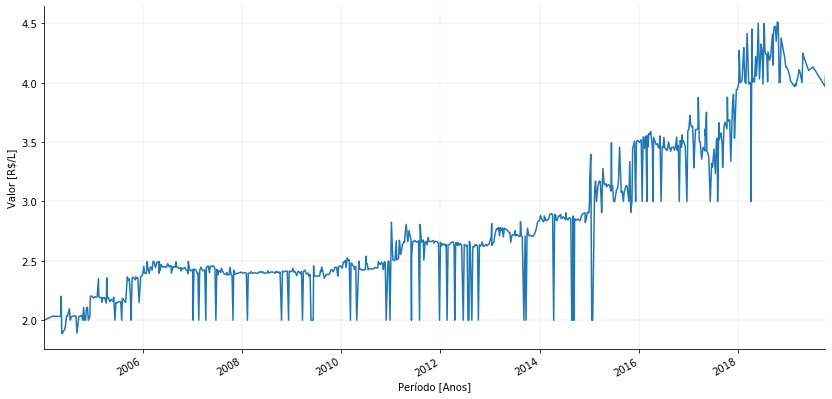
\includegraphics[width=1 \textwidth]{Figuras/precorevenda.png}
\fonte{Próprio autor}
\end{figure}

O gráfico da figura \ref{heatmap} mostra o mapa de calor(\textit{heatmap}) para as \textit{features} não repetidas do \textit{dataset}, ou seja, os valores temporais não são considerados nessa análise. Pela análise do gráfico conclui-se que apenas os coeficientes de variação não são relevantes o bastante para os modelos, os demais valores possuem fortíssima correlação com o preço médio de revenda.

\begin{figure}[!ht]
\centering
\caption{Gráfico de calor da correlação de \textit{features} do \textit{dataset}}
\label{heatmap}
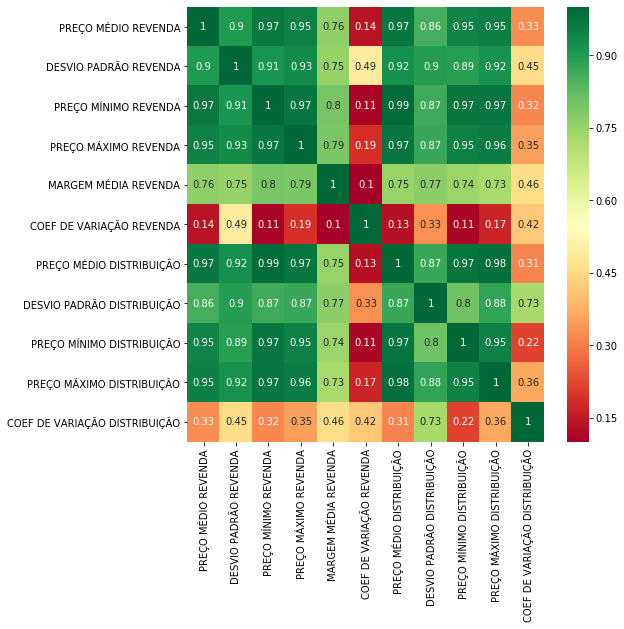
\includegraphics[width=1 \textwidth]{Figuras/heatmap.png}
\fonte{Próprio autor}
\end{figure}

\subsection{Modelos}

Métodos de aprendizado de máquina são em geral aplicados para problemas de regressão(\textit{regression}), classificação(\textit{classification}), redução de ordem(\textit{dimensionally reduction}) e agregação(\textit{clustering}). Previsão de uma série temporal, no caso o preço do combustível, caracteriza-se por um problema de regressão\cite{Eletricity}.

Este trabalho faz uso de alguns dos mais amplamente utilizados  algoritmos de regressão,
são eles \textit{Simple Linear Regression}, \textit{Ridge Regression}, \textit{Support Vector Regression} com \textit{kernel Linear}
e \textit{Radial basis function}\cite{Price}.

Os métodos anteriormente citados foram implementados utilizando a linguagem de programação Python em conjunto com as bibliotecas open sources
\textit{Python Data Analysis Library}(pandas) e \textit{scikit-learn}, a primeira permite o tratamento de dados  como transformação de texto para números e checagem de nível de correlação,
a segunda biblioteca é voltada para aprendizado de máquinas, esta possui os modelos e outras ferramentas utilitárias como
\textit{cross validation}.

Inicialmente separou-se o \textit{dataset} utilizando a biblioteca pandas, limitando-se aos já citados
dados que caracterizariam o problema, data,preço médio de revenda e preço médio de distribuição, também utilizando esta biblioteca foi adicionado a coluna \textit{label} que representa o \textit{target} deste trabalho, o preço de revenda.

Posteriormente, utilizando a biblioteca \textit{scikit-learn} o \textit{dataset} foi dividido em 
teste e treino na proporção 20\% para 80\%. O \textit{dataset} de treinamento foi utilizado para o
treinamento dos modelos. Pós treinamento, a notas de acurácia e os valores
de \textit{cross-validation} foram analisados para checar a precisão do modelo e garantir que não houve \textit{overfitting} durante o treinamento.

\section{Resultados}
A Tabela \ref{results} apresenta os resultados  obtidos do grupo de teste contra o modelo para os quadros modelos
escolhidos após o treinamento, também apresenta o resultado do \textit{cross validation} com 5 iterações de cruzamento (cv).
Observando os resultados adquiridos é notável que os valores para \textit{Linear Regression}  são muito superiores aos para os outro modelos, e que \textit{Ridge Regression} obteve resultados ligeiramente  melhores que o \textit{State Vector Regression} para ambos os kernels.

\begin{table}[!ht]
\centering
    \caption{Valores do treinamento}
    \label{results}
\begin{tabular}{c c c}
    Modelo & resultado & resultado em cross validation (cv=5) \\
    \hline
    Linear Regression & 0.62 & -0.23,  0.27,  0.85,  0.89,  -0.73 \\
    SVR (linear) & 0.01 & -0.76, -0.44,  0.016, -0.023, -1.45 \\
    Ridge & 0.61 & -0.18,  0.30, 0.86,  0.88, -0.76 \\
    SVR (rbf) & 0.01 & -0.76, -0.44,  0.016, -0.022, -1.45
\end{tabular}   
\fonte{Próprio autor}
\end{table}

Entretanto, o objetivo não era ver o ajuste de novos dados dentro do universo esperado, mas sim se os mesmo poderiam se previsto, para tanto foram utilizados os valores das trintas últimas semanas. O gráfico \ref{predict} apresenta os resultados para a predição, apesar do excelente \textit{score} obtido pelo  \textit{Linear Regression} o mesmo não foi capaz de prever com extrema confiança o valor do preço do combustível, ficando ligeiramente abaixo que os valores realmente praticados. Quanto ao demais modelos, estes apresentaram resultados pouco efetivos destoando muito do preço esperado.

Interessante notar que o SVR para o \textit{kernel} rbf apresenta um formato de curva muito parecido com o do preço esperado, porém o mesmo é muito sensível ao ruído apresentado no gráfico da imagem \ref{dataset-graph}, logo, o seu resultado não condiz com o esperado.


\begin{figure}[!ht]
\centering
\caption{Gráfico do valores do \textit{dataset} e dos obtidos por \textit{Linear Regression} e \textit{Rigid Regression}}
\label{predict}
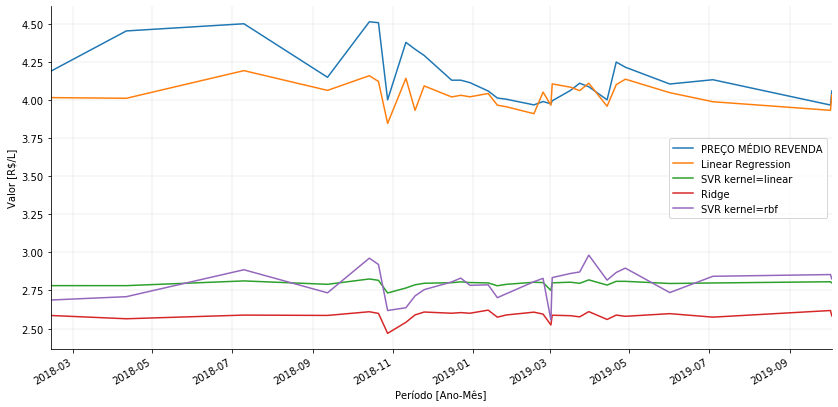
\includegraphics[width=1 \textwidth]{Figuras/predict.png}
\fonte{Próprio autor}
\end{figure}
% ---
\bookmarksetup{startatroot}% 
% ---

% ---
% Conclusão
% ---
\section{Considerações finais}
Por meio da análise dos resultados obtidos é notável que os modelos de regressão não são capazes de predizer
os valores dos combustíveis. Provavelmente devido a natureza de como o preço do combustível é definido, dependo
muito menos da produção e muito mais das interferências políticas, portanto, seria necessário uma análise 
de outro fatores como por exemplo o valor do combustível internacionalmente e das decisões tomadas 
pelo o Estado durante o período, este último dificilmente aplicável a um modelo de aprendizado de máquina, além de questões envolvendo a extração do petróleo.

Também é notável que os dados possuem muito ruído, é difícil saber se é apenas ruído devido a uma coleta ruim ou se 
é um padrão esperado quando medidas governamentais são tomadas para amenizar o preço ou por interesses do mercado. Além do mais, a homogeneidade dos dados é questionável em suas coletas, como por exemplo o número de postos por estado não é o mesmo, isto torna os dados desafiador julgar a qualidade dos dados.

Fica para trabalhos futuros adicionar as já citadas características políticas do preço, estas adicionariam camadas de complexidade à análise desta forma sendo capaz de cobrir a natureza do ruído do \textit{dataset}.



% ----------------------------------------------------------
% ELEMENTOS PÓS-TEXTUAIS
% ----------------------------------------------------------
\postextual

\clearpage
\bibliographystyle{abntex2-alf} 
\bibliography{Bib.bib}

\end{document}
